\documentclass[letterpaper]{article}
\usepackage[margin=1in]{geometry}
\usepackage[utf8]{inputenc}
\usepackage{textcomp}
\usepackage{amssymb}
\usepackage{natbib}
\usepackage{graphicx}
\usepackage{gensymb}
\usepackage{amsthm, amsmath, mathtools}
\usepackage[dvipsnames]{xcolor}
\usepackage{enumerate}
\usepackage{mdframed}
\usepackage[most]{tcolorbox}
\usepackage{csquotes}
% https://tex.stackexchange.com/questions/13506/how-to-continue-the-framed-text-box-on-multiple-pages

\tcbuselibrary{theorems}

\newcommand{\R}{\mathbb{R}}
\newcommand{\Z}{\mathbb{Z}}
\newcommand{\N}{\mathbb{N}}
\newcommand{\Q}{\mathbb{Q}}
\newcommand{\C}{\mathbb{C}}
\newcommand{\code}[1]{\texttt{#1}}
\newcommand{\mdiamond}{$\diamondsuit$}
\newcommand{\PowerSet}{\mathcal{P}}
\newcommand{\Mod}[1]{\ (\mathrm{mod}\ #1)}
\DeclareMathOperator{\lcm}{lcm}

%\newtheorem*{theorem}{Theorem}
%\newtheorem*{definition}{Definition}
%\newtheorem*{corollary}{Corollary}
%\newtheorem*{lemma}{Lemma}
\newtheorem*{proposition}{Proposition}


\newtcbtheorem[number within=section]{theorem}{Theorem}
{colback=green!5,colframe=green!35!black,fonttitle=\bfseries}{th}

\newtcbtheorem[number within=section]{definition}{Definition}
{colback=blue!5,colframe=blue!35!black,fonttitle=\bfseries}{def}

\newtcbtheorem[number within=section]{corollary}{Corollary}
{colback=yellow!5,colframe=yellow!35!black,fonttitle=\bfseries}{cor}

\newtcbtheorem[number within=section]{lemma}{Lemma}
{colback=red!5,colframe=red!35!black,fonttitle=\bfseries}{lem}

\newtcbtheorem[number within=section]{example}{Example}
{colback=white!5,colframe=white!35!black,fonttitle=\bfseries}{def}

\newtcbtheorem[number within=section]{note}{Important Note}{
        enhanced,
        sharp corners,
        attach boxed title to top left={
            xshift=-1mm,
            yshift=-5mm,
            yshifttext=-1mm
        },
        top=1.5em,
        colback=white,
        colframe=black,
        fonttitle=\bfseries,
        boxed title style={
            sharp corners,
            size=small,
            colback=red!75!black,
            colframe=red!75!black,
        } 
    }{impnote}
\usepackage[utf8]{inputenc}
\usepackage[english]{babel}
\usepackage{fancyhdr}
\usepackage[hidelinks]{hyperref}
\usepackage{pdflscape}

\fancypagestyle{noheader}{
  \fancyhf{}% Clear header/footer
  \renewcommand{\headrulewidth}{0pt}% No header rule
  \rfoot{\thepage}
} 

\pagestyle{fancy}
\fancyhf{}
\rhead{CSE 131}
\chead{Wednesday, May 31, 2023}
\lhead{Lecture 25}
\rfoot{\thepage}

\setlength{\parindent}{0pt}

\begin{document}

\section{Optimization (Continued)}
\subsection{Flow Analysis}
Let's consider the following code, 
\begin{verbatim}
    (let (curr lst)
        (let (total 0)
            (loop
                (if (= lst nil) (break total)
                    (block
                    (set! total (+ total (fst lst)))
                    (set! lst (snd lst)))))))\end{verbatim}
How can we use flow analysis to reduce the amount of tag checking generated in the final assembly?

\subsubsection{The \code{check} Instruction}
An idea we want to do is to make tag checks explicit with \code{check} steps: which checks can we remove? One new step we can introduce in the intermediate representation is 
\begin{verbatim}
    check <some bool expr>\end{verbatim} 
The semantics are simple: if the check is true, then everything continues as normal. Otherwise, an error is thrown.
\begin{mdframed}
    (Example.) \code{check sametag(curr, nil)} checks to see if \code{curr} has the same tag as \code{nil}. Something we've incorporated into our compiler is the \code{isnum(x)} and \code{isbool(x)} checks, which checks to see if the expression $x$ is a number or boolean, respectively.
\end{mdframed}
With this said, the corresponding intermediate representation of the above code is 
\begin{verbatim}
sum(lst) {
    start0:     curr <- lst
    start1:     total <- 0
    loop_0:     check sametag(curr, nil)
    loop_1:     %t_0 <- curr == nil
    loop_2:     if %t_0 thn_0 els_0
    thn_0:      rax <- total
    thn_1:      goto end_0
    thn_2:      goto ifend_0
    els_0:      check isnonnilpair(curr)
    els_1:      %t_1 <- fst curr
    els_2:      check isnum(total)
    els_3:      check isnum(%t_1)
    els_4:      %t_2 <- total + %t_1
    els_5:      total <- %t_2
    els_6:      check isnonnilpair(curr)
    els_7:      %t_3 <- snd curr
    els_8:      curr <- %t_3
    els_9:      rax <- curr
    els_10:     goto ifend_0
    ifend_0:    goto loop_0
    end_0:      return rax
}\end{verbatim}
We can use flow analysis to analyze how data flows through a program. We can use this information to identify variables that hold values at different points in the program, and how these values change over time. For our purposes, we wish to use flow analysis to reduce the amount of unncessary tag checking. Using the \code{check} instruction that was mentioned, we can do just this.

\newpage 
\thispagestyle{noheader}
\newgeometry{left=0.1in,right=0.1in,top=0.2in,bottom=0.5in}
\subsubsection{A Flow Analysis Walkthrough}
The flow analysis we'll do starts from the beginning and goes to the end (this is known as \emph{forward analysis}). The information we'll keep track of are the \emph{potential} tags. Let's analyze each line of the intermediate representation. For each line executed, we consider what possible tag value each variable can represent. The potential tags are \textbf{N}umbers, \textbf{B}ooleans, \textbf{Nil}, and \textbf{P}airs. At any point in the program, each variable can hold a set of these possible types. Let $A = \{N, B, \text{Nil}, P\}$ be the set of all types.

\begin{center}
    \begin{tabular}{p{2.5in}|p{0.48in}|p{0.82in}|p{0.48in}|p{0.48in}|p{0.48in}|p{0.48in}|p{0.48in}|p{0.48in}}
        IR & \code{lst} & \code{curr} & \code{total} & $t_0$ & $t_1$ & $t_2$ & $t_3$ & \code{rax} \\ 
        \hline  
        \hline 
        \verb|start0:  curr <- lst|                 & A & $\to A$  &   &   &   &   &   &   \\
        \hline
        \verb|start1:  total <- 0|                  & A & A  & $\to N$ &   &   &   &   &   \\
        \hline
        \verb|loop_0:  check sametag(curr, nil)|    & A  & $\to \{\text{Nil}, P\}$ & N &   &   &   &   &   \\
        \hline
        \verb|loop_1:  %t_0 <- curr == nil|         & A & $\{\text{Nil}, P\}$ & N & $\to B$ &   &   &   &   \\
        \hline
        \verb|loop_2:  if %t_0 thn_0 els_0|         & A & $\{\text{Nil}, P\}$  & N & B &   &   &   &   \\
        \hline
        \verb|thn_0:   rax <- total|                & A & \{\text{Nil}, P\} & N & B &   &   &   & N \\
        \hline
        \verb|thn_1:   goto end_0|                  & A & \{\text{Nil}, P\} & N & B &   &   &   & N \\
        \hline
        \verb|thn_2:   goto ifend_0|\footnote{}     &    &   &   &   &   &   &   &   \\
        \hline
        \verb|els_0:   check isnonnilpair(curr)|\footnote{}  & A & $\{\text{Nil}, P\} \to P$  & N & B &   &   &   &   \\
        \hline
        \verb|els_1:   %t_1 <- fst curr|            & A & P & N & B & $\to A$ &   &   &   \\
        \hline
        \verb|els_2:   check isnum(total)|          & A & P & $N \to N$ & B & $\to A$ &   &   &   \\
        \hline
        \verb|els_3:   check isnum(%t_1)|           & A & P & N & B & $A \to N$ &   &   &   \\
        \hline
        \verb|els_4:   %t_2 <- total + %t_1|        & A & P & N & B & N & $\to N$  &   &  \\
        \hline
        \verb|els_5:   total <- %t_2|               & A & P & $N \to N$ & B & N & N  &   &    \\
        \hline
        \verb|els_6:   check isnonnilpair(curr)|    & A & $P \to P$ & N & B & N & N  &   &    \\
        \hline
        \verb|els_7:   %t_3 <- snd curr|            & A & P & N & B & N & N  & $\to A$ &   \\
        \hline
        \verb|els_8:   curr <- %t_3|                & A & $P \to A$ & N & B & N & N  & A &   \\
        \hline
        \verb|els_9:   rax <- curr|                 & A & A & N & B & N & N & A & $\to A$ \\
        \hline
        \verb|els_10:  goto ifend_0|                & A & A & N & B & N & N & A & A \\
        \hline
        \verb|ifend_0: goto loop_0|                 & A & A & N & B & N & N & A & A \\
        \hline
        \verb|end_0:   return rax|                  &   &   &   &   &   &   &   &   \\
    \end{tabular}
\end{center}
\textbf{Remarks:}
\begin{itemize}
    \item At (1), we have dead code. So, nothing needs to be filled out.
    \item At (2), we can copy the tag information we have from the \code{goto} instruction which jumps to this line. In this case, we copied this information from the line \code{loop\_2}.
    \item In general, we can copy the information from the \code{goto} to the target label. This is especially important when we have a \code{goto} that goes to a label that's \emph{before} where the \code{goto} occurred.
\end{itemize}
At \code{goto loop\_0}, we now perform a backwards jump back to the label \code{loop\_0} and perform additional forward analysis with the information we found prior to the \code{goto}. These tags are denoted by red.
\begin{center}
    \begin{tabular}{p{2.5in}|p{0.48in}|p{0.82in}|p{0.48in}|p{0.48in}|p{0.48in}|p{0.48in}|p{0.48in}|p{0.48in}}
        IR & \code{lst} & \code{curr} & \code{total} & $t_0$ & $t_1$ & $t_2$ & $t_3$ & \code{rax} \\ 
        \hline  
        \hline 
        \verb|start0:  curr <- lst|                 & A & $\to A$  &   &   &   &   &   &   \\
        \hline
        \verb|start1:  total <- 0|                  & A & A  & $\to N$ &   &   &   &   &   \\
        \hline
        \verb|loop_0:  check sametag(curr, nil)|    & A  & $\textcolor{red}{A} \to \{\text{Nil}, P\}$ & N & \textcolor{red}{$\to B$} & \textcolor{red}{$\to N$}  & \textcolor{red}{$\to N$} & \textcolor{red}{$\to A$} & \textcolor{red}{$\to A$} \\
        \hline
        \verb|loop_1:  %t_0 <- curr == nil|         & A & $\{\text{Nil}, P\}$ & N & $\to B$ & \textcolor{red}{N}  & \textcolor{red}{N} & \textcolor{red}{A} & \textcolor{red}{A} \\
        \hline
        \verb|loop_2:  if %t_0 thn_0 els_0|         & A & $\{\text{Nil}, P\}$  & N & B & \textcolor{red}{N}  & \textcolor{red}{N} & \textcolor{red}{A} & \textcolor{red}{A} \\
        \hline
        \verb|thn_0:   rax <- total|                & A & \{\text{Nil}, P\} & N & B & \textcolor{red}{N}  & \textcolor{red}{N} & \textcolor{red}{A} & $\textcolor{red}{A} \to N$ \\
        \hline
        \verb|thn_1:   goto end_0|                  & A & \{\text{Nil}, P\} & N & B & \textcolor{red}{N}  & \textcolor{red}{N} & \textcolor{red}{A} & N \\
        \hline
        \verb|thn_2:   goto ifend_0|     &    &   &   &   &   &   &   &   \\
        \hline
        \verb|els_0:   check isnonnilpair(curr)|\footnote{}  & A & $\{\text{Nil}, P\} \to P$  & N & B & \textcolor{red}{N}  & \textcolor{red}{N} & \textcolor{red}{A} & \textcolor{red}{A} \\
        \hline
        \verb|els_1:   %t_1 <- fst curr|            & A & P & N & B & $\to A$ &   &   &   \\
        \hline
        \verb|els_2:   check isnum(total)|          & A & P & $N \to N$ & B & $\to A$ &   &   &   \\
        \hline
        \verb|els_3:   check isnum(%t_1)|           & A & P & N & B & $A \to N$ &   &   &   \\
        \hline
        \verb|els_4:   %t_2 <- total + %t_1|        & A & P & N & B & N & $\to N$  &   &  \\
        \hline
        \verb|els_5:   total <- %t_2|               & A & P & $N \to N$ & B & N & N  &   &    \\
        \hline
        \verb|els_6:   check isnonnilpair(curr)|    & A & $P \to P$ & N & B & N & N  &   &    \\
        \hline
        \verb|els_7:   %t_3 <- snd curr|            & A & P & N & B & N & N  & $\to A$ &   \\
        \hline
        \verb|els_8:   curr <- %t_3|                & A & $P \to A$ & N & B & N & N  & A &   \\
        \hline
        \verb|els_9:   rax <- curr|                 & A & A & N & B & N & N & A & $\to A$ \\
        \hline
        \verb|els_10:  goto ifend_0|                & A & A & N & B & N & N & A & A \\
        \hline
        \verb|ifend_0: goto loop_0|                 & A & A & N & B & N & N & A & A \\
        \hline
        \verb|end_0:   return rax|                  &   &   &   &   &   &   &   &   \\
    \end{tabular}
\end{center}

\restoregeometry
\newpage 

\textbf{Remark:}
\begin{itemize}
    \item At (4), note that we're not directly copying $N$ from \code{thn\_1} to \code{els\_0}. Rather, we're copying the tag information from the \code{goto} instruction that jumps to this line. 
\end{itemize}
Let's consider the lines \verb|els_2: check isnum(total)| and \verb|els_6: check isnonnilpair(curr)|. Based on the forward analysis, these two lines of code are useless. Likewise, \verb|els_0: check isnonnilpair(curr)| could be \emph{optimized} (not removed) to check if \code{curr} is \code{nil}.

\subsubsection{In Summary}
In summary, the idea behind flow analysis is that there's really two steps: 
\begin{enumerate}
    \item Do the analysis and gather information 
    \item Rescan the program with that information and change the program to remove/optimize any code as needed. 
\end{enumerate}
The corresponding \textbf{control flow graph} looks like 
\begin{center}
    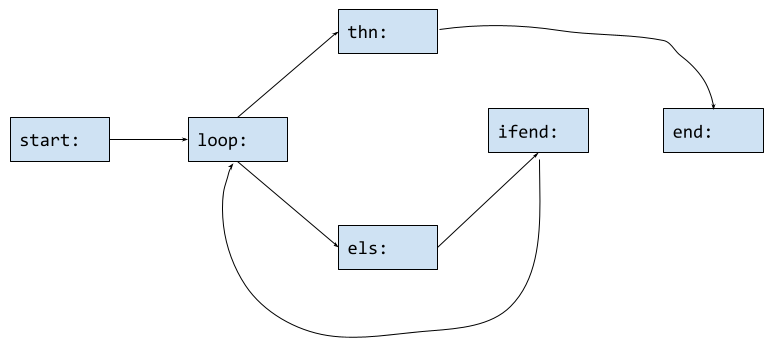
\includegraphics[scale=0.5]{../assets/analysis_flow_graph.png}
\end{center}
At the start, we have a bunch of instructions. This eventually leads to a loop. In the \code{thn} branch, we go straight to the end since we have the dead code. In the \code{els} branch, we eventually get to the \code{ifend} statement where we end up going to the loop.

\end{document}